\documentclass[conference,9pt,letterpaper]{IEEEtran}
\usepackage[T1]{fontenc}
\usepackage{newtxtext,newtxmath}
\usepackage{microtype}
\clubpenalty=10000
\widowpenalty=10000
\displaywidowpenalty=10000
\brokenpenalty=1000
\usepackage{graphicx}
\usepackage{booktabs}
\usepackage{amsmath}
\usepackage{array}
\usepackage{xcolor}
\usepackage{soul}
\DeclareRobustCommand{\pending}[1]{{\sethlcolor{yellow}\hl{#1}}}
\setlength{\abovecaptionskip}{3pt}
\setlength{\belowcaptionskip}{2pt}
\setlength{\intextsep}{6pt plus 1pt minus 1pt}
\setlength{\textfloatsep}{7pt plus 1pt minus 1pt}
\setlength{\floatsep}{6pt plus 1pt minus 1pt}
\usepackage{cite}
\usepackage{url}
\usepackage{stfloats}
\usepackage{balance}
\makeatletter
\patchcmd{\@BAlancecol}
 {\setbox\@leftcolumn=\vbox to \@tempdima}
 {\@tempdimb=\ht1\advance\@tempdimb by\dp1
  \ifdim\@tempdimb>\@tempdima\@tempdima=\@tempdimb\fi
  \@tempdimb=\ht3\advance\@tempdimb by\dp3
  \ifdim\@tempdimb>\@tempdima\@tempdima=\@tempdimb\fi
  \setbox\@leftcolumn=\vbox to \@tempdima}
 {\typeout{MECC: balance packing includes split-box depth.}}
 {\errmessage{Failed to patch balanced-column packing}}
% Stretch section and figure spacing instead of leaving unequal column tails.
\patchcmd{\@BAlancecol}{\unvbox1\vfil}{\unvbox1}
 {\typeout{MECC: balanced left column uses body glue.}}
 {\errmessage{Failed to patch left balance tail}}
\patchcmd{\@BAlancecol}{\vfil}{}
 {\typeout{MECC: balanced right column uses body glue.}}
 {\errmessage{Failed to patch right balance tail}}
\makeatother
\usepackage{capt-of}
\usepackage{float}
\usepackage{needspace}
\setcounter{dbltopnumber}{3}
\renewcommand{\dbltopfraction}{0.85}
\renewcommand{\textfraction}{0.10}
\newcommand{\mecc}{\textsc{MECC}}
\newcommand{\BH}{B_{\mathrm H}}
\newcommand{\BC}{B_{\mathrm C}}
\newcommand{\KH}{K_{\mathrm H}}
\newcommand{\KC}{K_{\mathrm C}}
\newtheorem{proposition}{Proposition}
\title{MECC: Single-GPU MoE Inference with\protect\\Compiler-Guided Three-Tier Expert Caching}
% Anonymous review copy: no author names or affiliation spacer rows.
\author{}
\usepackage[hidelinks]{hyperref}
\hypersetup{pdftitle={MECC: Single-GPU MoE Inference with Compiler-Guided Three-Tier Expert Caching},pdfauthor={}}
\begin{document}
\maketitle\flushbottom
\begin{abstract}
Expert offloading enables single-GPU inference for mixture-of-experts (MoE) models. Repeated HDD reads make expert residency a source of inference latency. We present MECC, the MoE Expert Cache Compiler, for profile-guided placement and joint HBM/CPU caching. Its compiler allocates slots by layer and emits the expert IDs used for initialization. The runtime promotes router-selected experts and retains displaced GPU weights in the host cache. The delivery path orders HDD reads and H2D copies before GPU consumption. On one A100, MECC decodes FP16 Mixtral-8x7B at 7.38~s/token with uniform initialization. Decode speedups are 1.77$\times$ over streaming and 2.95$\times$ over fixed CPU retention, with matching perplexity.
\end{abstract}

\begin{IEEEkeywords}
Mixture of experts, single-GPU inference, expert offloading, three-tier caching, hardware/software co-design.
\end{IEEEkeywords}

\section{Introduction}
Mixture-of-experts (MoE) models scale parameter capacity through sparse expert activation~\cite{shazeer,switch,mixtral,deepseekmoe}. For example, Mixtral selects two of eight experts in each layer. A single-GPU deployment can use high-bandwidth memory (HBM), host memory, and a hard disk drive (HDD) to hold that pool. The selected expert's location then determines its delivery path. HBM residents are ready for GPU execution; host residents require a host-to-device (H2D) copy; cold experts require an HDD read followed by H2D. The next layer consumes the current layer's output, so an exposed read also delays downstream computation. Prefill can reuse one fetched expert across prompt rows, and decoding can reuse its weights across output tokens. Retaining the corresponding cache state avoids fetching those weights again. The placement problem is therefore tied to the request sequence, rather than to model loading alone. On shared servers, a serving task manages its expert allocation alongside other jobs and model instances. We study how to distribute that allocation across layers and preserve the resulting reuse during inference. All MoE layers share the HBM and host allowances. Increasing one layer's allocation leaves fewer slots for others. The value of another slot depends on the demand already covered in that layer. Placement therefore couples the layers' local request distributions to a shared storage allocation.



Expert parallelism places experts across GPUs~\cite{deepspeedmoe,tutel,flashmoedist}. Single-GPU systems combine expert paging and caching~\cite{offloading,swapmoe,moeinfinity,promoe} with CPU/GPU execution~\cite{fiddler,daop,lightning}. MoE-CORE combines layer-wise allocation, profile initialization, and online replacement with cross-layer prefetching~\cite{core}. It also supports substitution for eligible expert misses. SSD-LLaMA retains GPU victims in RAM and pipelines storage delivery alongside lossless compression and CPU/GPU work partitioning~\cite{ssdllama}. Edge FlashMoE studies cache replacement for storage-backed expert access~\cite{flashmoe}. Within such a hierarchy, initial placement and later admission affect different requests. A profile determines which weights are available when serving begins. GPU turnover then determines which of those weights survive on the host. Promoting a CPU expert vacates a host position just as an HBM victim loses its GPU position. Using that position for the victim preserves its place in the reuse order. Figure~\ref{fig:intro} compares this joint rule with independent HBM/CPU caches on an A100. Decode time is 7.38~s/token under joint retention and 32.94~s/token under independent replacement. HDD demand is 12.5\% versus 47.9\%. These results motivate compiling an initial resident set and preserving subsequent reuse across both tiers.



\begin{figure}[!t]
\centering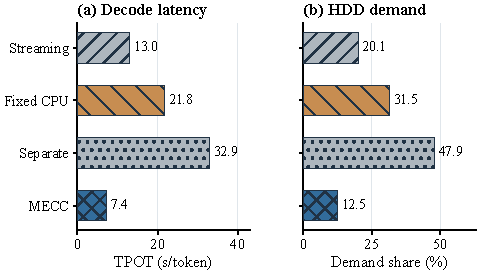
\includegraphics[width=\columnwidth]{measured_figures/intro_evidence.pdf}
\par\nointerlineskip
\caption{Single-A100 expert-cache comparison on Mixtral-8x7B. Separate uses independent HBM/CPU replacement. Joint retention lowers both plotted metrics.}
\label{fig:intro}
\end{figure}

We present \mecc{}, the MoE Expert Cache Compiler, to connect these two stages. Compilation ranks experts within each layer and allocates slots by marginal covered demand. The resulting plan specifies both per-layer capacities and the IDs loaded into HBM and CPU. The runtime then maintains a joint recency order across those tiers. A CPU hit promotes the selected expert and demotes the GPU victim; a cold admission can also evict a host resident. The runtime keeps a host mirror with each HBM resident and reuses that copy during demotion. Host admission therefore updates the cache metadata at that boundary. Consuming-stream tracking keeps the tensor storage live through kernel execution. This process keeps the capacities fixed while updating membership from the actual request stream. Weight delivery follows the selected experts' read and copy dependencies before GPU execution. Prefill submits cold reads for the active expert batch, while decode loads selected experts on demand. The same layer/expert identity passes from profiling through placement to execution, preserving the original router selections and FP16 computation.

This paper makes three contributions.
\begin{list}{}{\setlength{\leftmargin}{16pt}\setlength{\labelwidth}{14pt}\setlength{\labelsep}{2pt}\setlength{\itemsep}{3pt}\setlength{\topsep}{3pt}}
\item[(1)] \textbf{Compiling initial residency.} We map layer profiles and expert allowances to per-layer capacities and ranked expert IDs. A marginal-coverage scan determines how each additional slot extends the initial resident set.
\item[(2)] \textbf{Updating cross-tier residency.} We connect the compiled state to joint promotion and victim demotion. Host retention preserves GPU evictions for later reuse, while read/copy ordering prepares selected weights for consumption.
\item[(3)] \textbf{Evaluating weight delivery.} We compare placement, retention, and scheduling through decode latency, first-token time, source-tier demand, and sample perplexity. Workload and capacity sweeps examine calibration, task transfer, prompt length, batch size, and host allocation. Deployment comparisons report latency and accelerator occupancy.
\end{list}
\twocolumn[{
\begin{minipage}{\textwidth}
\centering
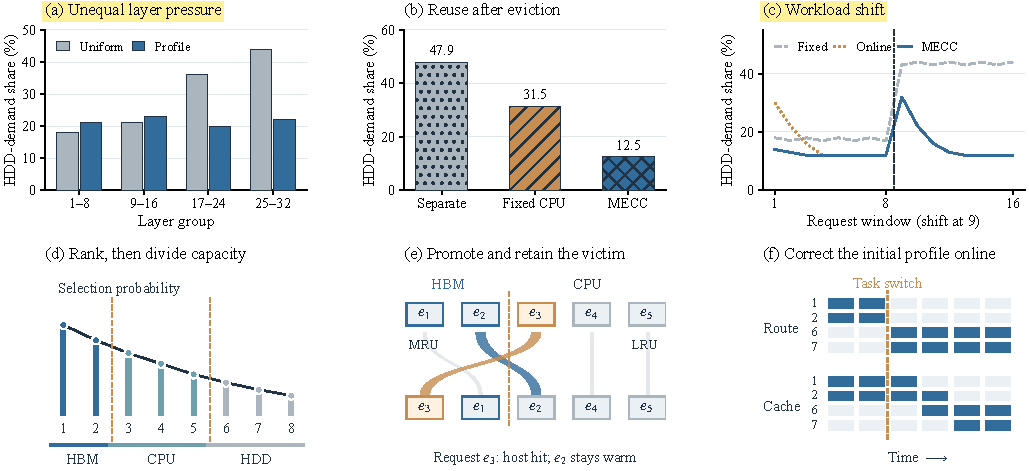
\includegraphics[width=\textwidth]{figures/fig02_motivation_insights.pdf}
\par\nointerlineskip
\captionof{figure}{Motivation evidence and matching insights. (a--c) compare layer pressure, cross-tier reuse, and workload change; (b) counts A100 demand across all phases. (d--f) show layer-specific capacity cuts, joint victim retention, and online membership updates.}
\label{fig:insights}
\vspace{5pt}
\end{minipage}
}]
\balance
\section{Background}
\label{sec:background}
\subsection{Sparse Execution, Full Weight Capacity}
An MoE layer routes each token to a subset of experts and combines their outputs~\cite{shazeer,switch,gshard}. Mixtral and the DeepSeek family separate active computation from the size of the stored expert pool~\cite{mixtral,deepseekmoe,deepseekv2,deepseekv3,mixtral22}. An expert belongs to one layer; equal indices at different layers identify different weights. For input $x$, let $G(x)$ be the selected set and $g_e(x)$ its normalized gate weights. The layer computes
\begin{equation}
y(x)=\sum_{e\in G(x)}g_e(x)E_e(x).
\end{equation}
A token traverses the MoE layers in order, revealing expert demand at each gate. Decoding revisits those layers for the next token. Caching changes the source of the selected weights while preserving the routing weights and expert functions.

\subsection{Expert Residency on One GPU}
Expert parallelism places experts on GPU owners and dispatches token activations to them~\cite{deepspeedmoe,tutel,megablocks,flashmoedist,harmoeny}. A single-GPU offloading system instead delivers selected weights to the execution device. Experts share HBM with dense weights, activations, and the KV cache~\cite{pagedattention,sglang}. The host cache supplies H2D copies; HDD supplies weights absent from both resident tiers. Heterogeneous inference systems combine these paths with CPU/GPU scheduling~\cite{flexgen,dsinference,zeroinfinity,llmflash,powerinfer,hetegen}. In prefill, several prompt rows can share a fetched expert. Decode advances one token per sequence, exposing fewer rows to each active expert. The amount of ready computation therefore changes between the two phases. Other systems change transfer size through precision selection~\cite{hobbit,specter}, expert segmentation~\cite{moepic,slicemoe}, or staging and compression~\cite{mira,zipmoe}.

Calibration counts determine expert ranking; runtime accesses determine recency. Within one layer, sequences $[a,a,b,b]$ and $[b,b,a,a]$ have equal counts and different last-access orders. MECC initializes from the ranked profile and replaces residents by recency.

\section{Motivation and Insights}
\label{sec:challenges}
\subsection{Allocating Slots by Marginal Demand}
Equal expert counts do not imply equal demand across layers. A few ranks may cover most requests in one layer, while another layer spreads requests over more experts. Figure~\ref{fig:insights}(a,d) illustrates the resulting allocation choice. Its profile-guided plan shifts slots toward the layer groups with more cold demand. The compiler makes this choice by comparing each layer's next uncovered rank. Allocating a slot exposes that layer's following rank as a new candidate. This process distributes a shared allowance across layers and retains the IDs that fill each allocation. Routing locality across models has also been studied independently~\cite{routingconsistency}.

\subsection{Preserving Reuse after GPU Eviction}
A GPU victim is also a candidate for host admission. Figure~\ref{fig:insights}(b,e) shows a CPU promotion vacating a host position as the GPU selects its victim. Joint retention admits that victim into the vacated position, carrying recency across the tier boundary. The independent-cache control reports 47.9\% HDD demand, compared with 12.5\% for the joint rule. Both start from the same allocation and expert order. The difference concerns how each policy retains the weights selected during execution. Preserving the victim lets a later selection use its host copy instead of initiating another cold read.

\subsection{Updating Residency beyond Calibration}
Calibration and serving inputs can select different expert sets. In Figure~\ref{fig:insights}(c,f), a task switch changes demand while preserving the cache capacities. The fixed placement continues to retain its original expert set. Online admission instead brings newly selected experts into the resident order. Profile initialization lowers the early demand transient, and online replacement follows the subsequent switch. These effects occur at different points in the same request sequence. MECC therefore initializes each resident set from the calibration profile. Runtime accesses then update its membership within the compiled per-layer capacities.

\twocolumn[{
\begin{minipage}{\textwidth}
\centering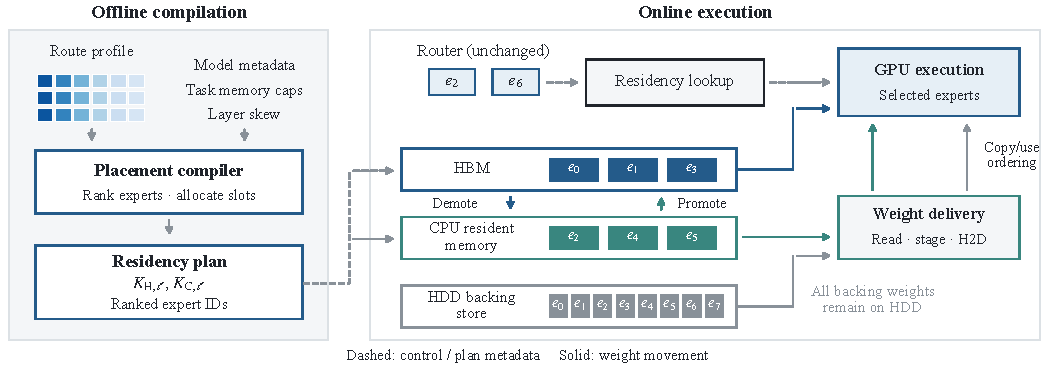
\includegraphics[width=\textwidth]{figures/fig01_overview.pdf}
\par\nointerlineskip
\captionof{figure}{MECC framework. The placement compiler emits per-layer capacities and ranked IDs. Online execution resolves unchanged router selections against HBM, CPU resident memory, and HDD, then delivers weights before their GPU consumers. Dashed arrows carry control or plan metadata; solid arrows move weights.}
\label{fig:overview}

\vspace{8pt}
\end{minipage}
}]

\nobalance
\section{Overview}
\label{sec:overview}
Figure~\ref{fig:overview} follows the plan from profiling to GPU execution. The compiler receives layer/expert counts, skew parameters, model metadata, and expert allowances. It emits capacities and ranked IDs for each layer. Initialization loads the corresponding HBM and CPU residents; the complete expert pool remains on HDD. The runtime subsequently consumes this plan as an initial cache state.

Consider the selected experts $e_2$ and $e_6$ in the framework. The residency lookup finds $e_2$ on the host and $e_6$ in the backing store. Promoting $e_2$ frees a host position for an HBM victim. Loading $e_6$ then admits another GPU resident and updates the same tier order. The delivery path resolves each weight's read and copy before its consumer executes. The model combines the expert outputs using the gate weights and continues to the next layer.

Residency persists across tokens. Each layer updates its own membership within the compiled capacities. The original layer/expert IDs continue to identify the same weights after promotion or eviction. Section~\ref{sec:method} describes the allocation and transition rules; Section~\ref{sec:evaluation} evaluates their effect on delivery.

\section{Method}
\label{sec:method}
\subsection{Compiling Capacities and Initial Identities}
\begin{figure}[H]
\centering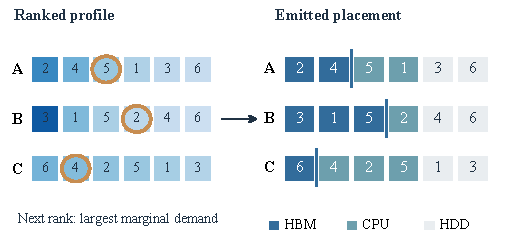
\includegraphics[width=\columnwidth]{method_redesign/compile_frontiers.pdf}
\par\nointerlineskip
\caption{Compiling the initial state. The left grid contains ranked per-layer demand; circles mark the next uncovered candidates. Shared HBM/CPU slot allowances produce different cuts in the emitted rows. A, B, and C identify different layers. }
\label{fig:compile}
\end{figure}

Consider $L$ MoE layers with $N_\ell$ experts per layer. Within each model, experts have equal size $s$ and layers use the same top-$k$.

Expert allowances $B_{\mathrm H}$ and $B_{\mathrm C}$ provide $S_{\mathrm H}=\lfloor B_{\mathrm H}/s\rfloor$ HBM slots and $S_{\mathrm C}=\lfloor B_{\mathrm C}/s\rfloor$ CPU slots.

For each layer, the compiler receives an expert order and a skew parameter $\alpha_\ell$. Profile counts determine the order. A discrete Zipf model gives the probability associated with each rank:
\begin{equation}
q_{\ell,r}=\frac{r^{-\alpha_\ell}}{\sum_{j=1}^{N_\ell}j^{-\alpha_\ell}},
\qquad p_{\ell,r}=q_{\ell,r}/L.
\end{equation}
Here $q_{\ell,r}$ is conditional on an access to layer $\ell$. Equal top-$k$ gives equal selection mass across layers. The ranked list preserves the original ID at each position.

Figure~\ref{fig:compile} shows the HBM and CPU cuts in those lists. Capacities satisfy $\sum_\ell K_{\mathrm H,\ell}\le S_{\mathrm H}$, $\sum_\ell K_{\mathrm C,\ell}\le S_{\mathrm C}$, and $K_{\mathrm H,\ell}+K_{\mathrm C,\ell}\le N_\ell$. The adaptive scan reserves one slot per layer in each fast tier, then distributes the remaining slots by marginal coverage.

The scan first assigns HBM slots. At each step, it chooses the layer with the largest next-rank score:
\begin{equation}
\Delta_\ell=q_{\ell,K_{\mathrm H,\ell}+1}.
\end{equation}
CPU allocation continues from the first ranks beyond each HBM cut. Every allocation exposes a new next-rank candidate in that layer. Layer ID breaks score ties, and expert ID breaks count ties. The direct scan takes $O(L(S_{\mathrm H}+S_{\mathrm C}))$ time after sorting. Its score is the request probability covered by the next slot.

The emitted plan contains the final capacities and ordered expert IDs. Initialization places each layer's first HBM ranks on the GPU and its next CPU ranks on the host. Natural ID order initializes the uniform control. During execution, admission changes membership within the compiled capacities.

\subsection{Retaining Victims across the Tier Boundary}
Each layer maintains two ordered sets, from most-recently used (MRU) to least-recently used (LRU). Their concatenation places HBM residents before CPU residents. An HBM hit moves its expert to HBM MRU. A CPU hit removes its host entry and promotes it to HBM MRU. The GPU LRU victim then becomes CPU MRU. A cold admission follows the same GPU insertion and can remove the CPU LRU. HDD retains the backing weights for every expert.

\begin{figure}[H]
\centering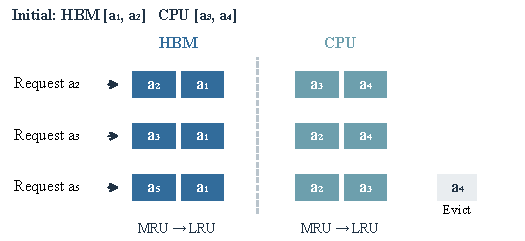
\includegraphics[width=\columnwidth]{method_redesign/residency_cases.pdf}
\par\nointerlineskip
\caption{Three requests from the same initial state. A hit changes recency; a host promotion also demotes the GPU victim; a cold admission can additionally evict the CPU victim. Rows show completed logical states, each ordered MRU to LRU.}
\label{fig:retention}
\end{figure}
Each row in Figure~\ref{fig:retention} starts from HBM $[a_1,a_2]$ and CPU $[a_3,a_4]$. An $a_2$ hit changes the GPU order. Promoting $a_3$ releases its CPU position, which receives the HBM victim $a_2$. A cold $a_5$ admission releases no CPU position. Retaining its GPU victim therefore removes the host LRU $a_4$. The two admission paths use the same demotion rule; their difference is the host space released by the request.

Completed serial transitions implement exclusive LRU over the combined resident capacity. Batch preparation can schedule several promotions before their consumers execute. Temporary copies bridge that preparation to the same ordered expert computation.

A host mirror accompanies each GPU resident and supplies its weights during demotion. Reusing that copy avoids a return transfer from the GPU. Cache eviction changes membership, while stream tracking keeps the underlying storage live through GPU consumption.

\subsection{Ordering Delivery before Expert Consumption}
Prefill groups token rows by selected expert and submits the corresponding cold reads. Each read is resolved when its expert reaches consumption. Figure~\ref{fig:delivery} shows resident work overlapping a pending read for another selected expert. Decode uses demand delivery. Both paths preserve the router's selected set and aggregation order.

\begin{figure}[H]
\centering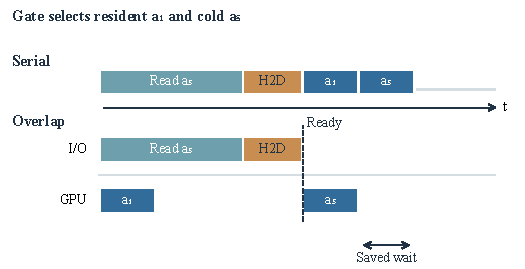
\includegraphics[width=\columnwidth]{method_redesign/delivery_overlap.pdf}
\par\nointerlineskip
\caption{Prefill delivery of resident $a_1$ and cold $a_5$ selected by one gate. Overlap executes ready work during the same read/copy path. The copy/use boundary orders $a_5$'s consumer; the host source remains live through copy completion. }
\label{fig:delivery}
\end{figure}
A completed read future supplies the host weights for H2D. The loader waits on the copy stream before yielding CUDA weights to a consumer. Recording that consumer's stream preserves tensor storage until its kernels finish. Read completion, copy synchronization, and storage lifetime therefore order the same selected expert from HDD to execution.

Prefetchers use profiles or lookahead to anticipate expert demand~\cite{pregated,fate,expertflow}. Batch and request schedulers expose work from concurrent inputs~\cite{klotski,bevy}; distributed edge schemes add network delivery~\cite{odmoe}. MECC schedules the expert work already selected at the current gate. Retention avoids a read or copy, whereas overlap reduces the time that the remaining delivery occupies the critical path.

\subsection{Sharing the Expert Execution Interface}
All policies use the same FP16 loader, model graph, and router. Layer/expert IDs resolve to weight tensors, while the router supplies the selected set and aggregation weights. A policy chooses residency and the source tier for each request. Delivery then prepares those tensors for the shared expert consumer.

\section{Evaluation}
\label{sec:evaluation}
\subsection{Evaluation Overview}
We report time per output token (TPOT), time to first token (TTFT), expert-demand classifications, and workload sensitivity. Placement, retention, and scheduling comparisons follow the corresponding method decisions. Deployment results report latency alongside accelerator occupancy. Appendix~\ref{app:setup} details hardware, policy settings, and measurement procedures.

\subsection{Single-GPU Performance}
\begin{figure}[H]
\centering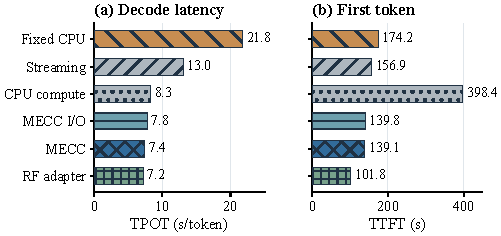
\includegraphics[width=\columnwidth]{measured_figures/main.pdf}
\par\nointerlineskip
\caption{Single-A100 runtime comparison. The panels report per-token decode time and time to first token.}
\label{fig:performance}
\end{figure}
Figure~\ref{fig:performance} reports 7.38~s/token for MECC, compared with 13.04 for streaming and 21.75 for fixed CPU retention. The corresponding decode speedups are 1.77$\times$ and 2.95$\times$. The recency/frequency (RF) adapter, MECC I/O, and CPU-compute take 7.19, 7.78, and 8.26~s/token. First-token time is 139.1~s for MECC, 156.9 for streaming, and 174.2 for fixed CPU. Perplexity (PPL) is 3.427 for the GPU-execution policies and 3.432 for CPU-compute. The latency rankings differ across phases. CPU-compute approaches the GPU policies during decode, yet its first-token time reaches 398.4~s. Short responses give this initial phase more weight; longer responses expose the recurring cost of expert delivery.

The access mix distinguishes the MECC and RF policies. MECC records 77.5\% HBM, 10.0\% CPU, and 12.5\% HDD demand; RF records 52.2\%, 36.6\%, and 11.1\%. RF trades a smaller HBM share for more host hits and takes 7.19~s/token, compared with MECC's 7.38. A host hit adds an H2D copy but avoids an HDD read. A GPU hit avoids both operations. The relevant distinction is therefore where each miss is served, rather than the HBM-hit fraction alone. Both policies use the same FP16 expert execution path. The comparison links residency to the cost of supplying selected weights.

\begin{figure*}[!t]
\centering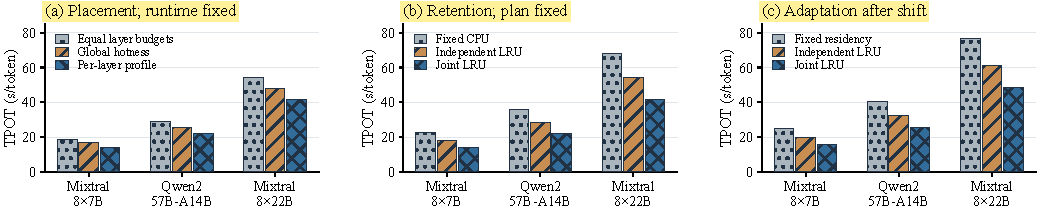
\includegraphics[width=\textwidth]{completion_figures/mechanism_sweeps.pdf}
\par\nointerlineskip
\caption{Component comparisons on three models. (a) Placement with runtime fixed. (b) Retention with initialization fixed. (c) Adaptation after a task switch. }
\label{fig:target_mechanisms}
\end{figure*}
\Needspace*{12\baselineskip}
\subsection{Mechanism Attribution}
\label{sec:mechanisms}

Figure~\ref{fig:target_mechanisms} varies one decision in each panel. The placement comparison keeps the runtime rule fixed; retention keeps initialization fixed; adaptation follows a task switch. For Mixtral-8x7B, per-layer placement changes TPOT from \pending{18.6 to 14.2 s/token}. Joint retention changes it from \pending{18.3 to 14.2}, and online adaptation changes the post-switch value from \pending{25.1 to 16.0}. The same comparisons span three models, relating each mechanism to its allocation or request sequence.

\begin{figure}[H]
\centering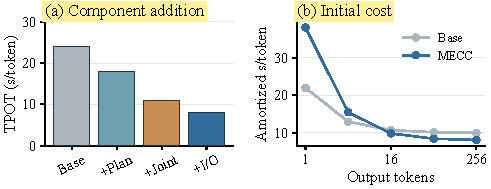
\includegraphics[width=\columnwidth]{completion_figures/ablation_startup.pdf}
\par\nointerlineskip
\caption{Ablation and startup. The right panel reports initialization cost per output token plus decode cost.}
\label{fig:target_ablation}
\end{figure}
Adding placement, joint retention, and I/O scheduling gives the TPOT sequence \pending{24, 18, 11, and 8 s/token} in Figure~\ref{fig:target_ablation}(a). The successive reductions are \pending{6, 7, and 3 s/token}. Joint retention provides the largest step by keeping GPU victims available on the host. Scheduling adds a further reduction while preserving HDD demand at \pending{20 percent}. Panel (b) includes the initial placement cost, connecting this decode gain to the response length.

\begin{figure}[H]
\centering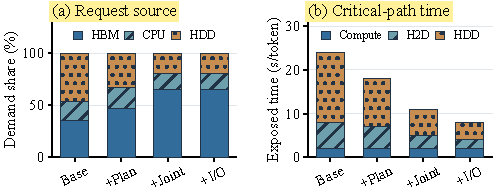
\includegraphics[width=\columnwidth]{completion_figures/traffic_exposure.pdf}
\par\nointerlineskip
\caption{Source demand and exposed time. The last I/O step preserves the demand fractions while shortening the exposed read/copy path.}
\label{fig:target_traffic}
\end{figure}
Figure~\ref{fig:target_traffic} separates changes in demand from changes in exposed time. Placement and joint retention lower HDD demand from \pending{46 to 20 percent}. The final I/O step leaves the HBM/CPU/HDD mix at \pending{65/15/20 percent}. Its TPOT reduction from \pending{11 to 8 s/token} comprises \pending{2 seconds} less exposed HDD time and \pending{1 second} less exposed H2D time. The compute component remains at \pending{2 seconds}. This step changes when transfers finish relative to ready computation; it does not require another reduction in cold requests. The breakdown distinguishes avoiding transfers through retention from overlapping the transfers that remain.

\subsection{Model and Deployment Scaling}
\begin{figure}[H]
\centering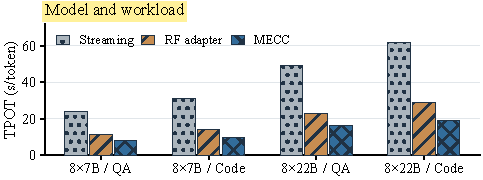
\includegraphics[width=\columnwidth]{completion_figures/cross_model.pdf}
\par\nointerlineskip
\caption{Model and workload comparison. Mixtral-8x7B and 8x22B with QA/code inputs. Each policy uses the same model and workload within a group. }
\label{fig:target_models}
\end{figure}
In Figure~\ref{fig:target_models}, MECC's speedup over streaming spans \pending{3.00--3.26}$\times$ across the four model/workload groups. The absolute TPOT difference grows from \pending{16 seconds} on 8x7B QA to \pending{43 seconds} on 8x22B Code. Moving from 8x7B to 8x22B \pending{doubles} MECC TPOT; the corresponding streaming increase is \pending{2.00--2.04}$\times$. Thus the larger model preserves the relative delivery gain while saving more time per token.

\begin{figure}[H]
\centering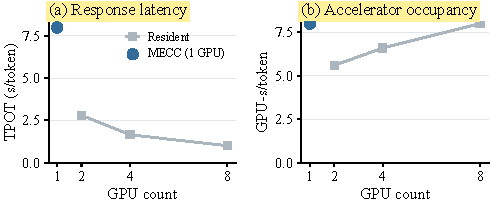
\includegraphics[width=\columnwidth]{completion_figures/gpu_tradeoff.pdf}
\par\nointerlineskip
\caption{One-GPU/resident-reference tradeoff. The panels compare single-GPU MECC with resident configurations and report latency alongside GPU occupancy.}
\label{fig:target_gpu}
\end{figure}
The endpoints in Figure~\ref{fig:target_gpu} pair \pending{one GPU at 8 s/token with eight GPUs at 1 s/token}. Both use \pending{8 GPU-s/token}, with different response times. The \pending{two-GPU resident point uses 5.6 GPU-s/token}. Plotting the intermediate configurations shows how accelerator provisioning changes both latency and occupancy. The single-GPU point quantifies the latency of supplying weights through the memory hierarchy.

\begin{figure*}[!t]
\centering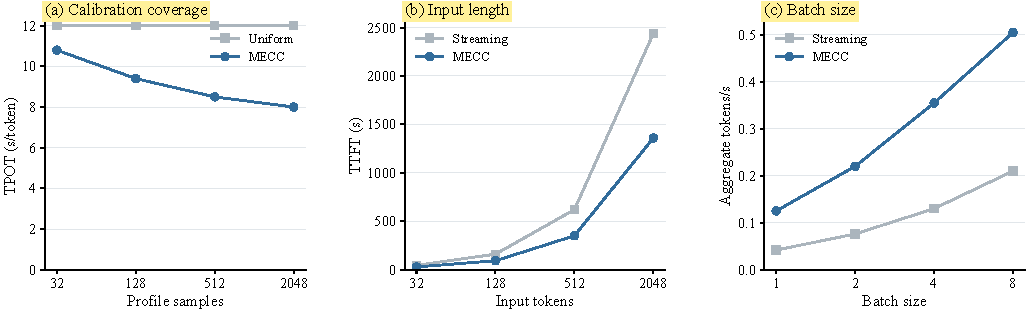
\includegraphics[width=\textwidth]{completion_figures/workload_sensitivity.pdf}
\par\nointerlineskip
\caption{Profile, input-length, and batch sensitivity. Profile size changes initialization quality, input length changes first-token work, and batch size changes aggregate throughput. The panels vary one workload parameter at a time.}
\label{fig:target_sensitivity}
\end{figure*}
\subsection{Capacity and Workload Sensitivity}

At 30 and 60~GB, MECC takes 14.46 and 0.76~s/token; RF takes 13.06 and 0.74. MECC's HDD demand falls from 32.2\% to zero. At 60~GB, all eight experts per layer fit in the resident tiers.

\begin{figure}[H]
\centering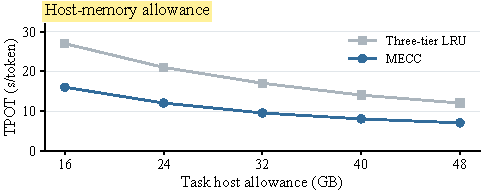
\includegraphics[width=\columnwidth]{completion_figures/quota_targets.pdf}
\par\nointerlineskip
\caption{Decode latency across host-memory allowances.}
\label{fig:target_quota}
\end{figure}
Figure~\ref{fig:target_quota} resolves the capacity range between sparse and broader host retention. MECC changes from \pending{16 to 7 s/token} across \pending{16--48 GB}; three-tier LRU changes from \pending{27 to 12}. The first host increment saves \pending{4 seconds/token} for MECC, while the final increment saves \pending{1 second/token}. Earlier slots can retain victims with shorter reuse distances. Additional slots then cover less frequent returns. This diminishing latency reduction complements the coverage transition at 60~GB, where the primary resident sets contain every expert.

\begin{figure}[H]
\centering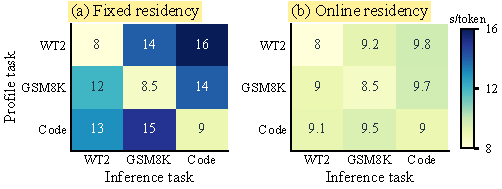
\includegraphics[width=\columnwidth]{completion_figures/profile_mismatch.pdf}
\par\nointerlineskip
\caption{Profile transfer across tasks. Rows select the calibration task and columns the inference task. Cells are TPOT in s/token; the two panels share a color scale.}
\label{fig:target_mismatch}
\end{figure}
Figure~\ref{fig:target_mismatch} separates within-task calibration from transfer to another task. The mean diagonal TPOT is \pending{8.50 s/token} under both fixed and online residency. Across the six off-diagonal pairs, the mean changes from \pending{14.00 to 9.38 s/token}, a \pending{33.0 percent} reduction. Online admission therefore recovers cross-task reuse while retaining the same-task values shown on the diagonal. The response to calibration size in Figure~\ref{fig:target_sensitivity}(a) addresses a different effect: how much profile information is available before the first request.

\balance
\subsection{Calibration Coverage and Input Length}
Increasing calibration from \pending{32 to 2048 samples} changes TPOT from \pending{10.8 to 8.0 s/token} in Figure~\ref{fig:target_sensitivity}(a). The final expansion yields a smaller reduction than the first. Once the ranked hot set stabilizes, additional samples affect fewer initial placements.

Figure~\ref{fig:target_sensitivity}(b) scales the prompt from \pending{32 to 2048 tokens}. MECC's TTFT changes from \pending{28 to 1360 seconds}, compared with \pending{45 to 2440} for streaming. Their endpoint speedups are \pending{1.61}$\times$ and \pending{1.79}$\times$. Prompt rows selected for the same expert can share one fetched weight block. Increasing input length thus exposes more opportunities to amortize delivery within prefill, alongside the increase in prompt computation.

\subsection{Batch Throughput and Sequence Progress}
Figure~\ref{fig:target_sensitivity}(c) reports aggregate output rate. Moving from \pending{one to eight sequences} increases MECC throughput from \pending{0.125 to 0.505 tokens/s}, or \pending{4.04}$\times$. The additional sequences share fetched expert weights and introduce more active rows at each gate.

For a synchronous batch of $B$ sequences with aggregate rate $R(B)$, the interval between batch steps is $B/R(B)$. The plotted MECC rates give \pending{8.00 seconds} at batch one and \pending{15.84 seconds} at batch eight. Batching therefore processes more tokens per unit time while increasing the interval between successive tokens of one sequence.

\subsection{Amortizing Initial Placement}
\label{sec:amortization}
Let $\Delta I$ denote the extra initialization time and $\Delta D$ the per-token decode saving. Equating the amortized per-token times gives the crossing $n^\star=\Delta I/\Delta D$. Figure~\ref{fig:target_ablation}(b) uses \pending{18 seconds} of extra initialization and \pending{2 seconds} of decode saving, yielding \pending{9 output tokens}. Longer responses recover the placement cost and retain part of the decode gain.

At \pending{64 output tokens}, initialization contributes \pending{0.47 s/token} for MECC and \pending{0.19} for the reference. Their total averages become \pending{8.47 and 10.19 s/token}, respectively. When requests share a resident cache, their output tokens amortize the same initialization. The relevant horizon is the cache lifetime, rather than one prompt.

\section{Conclusion}
MECC combines profile-guided initial placement with joint HBM/CPU retention for single-GPU MoE inference. Its allocation and admission rules reduce repeated weight delivery, while scheduling overlaps the remaining read/copy work with ready expert computation. The A100 comparison reports 7.38~s/token at matched PPL.

\clearpage
\balance
\bibliographystyle{IEEEtran}
\bibliography{references}
\clearpage
\appendices
\balance
\section{Experimental Configuration and Figure Data}
\label{app:setup}
\subsection{Hardware and Weight Representation}
The measured testbed uses one NVIDIA A100 80~GB PCIe. Expert weights use FP16. Dense layers and the router execute on the GPU. The expert store resides on a RAID logical volume reporting rotational media through ROTA=1. The manuscript calls this backing tier HDD. The logical-device record identifies the exposed storage path; the controller's physical-drive inventory is a separate platform record.

Each stored expert contains its gate, up, and down weight tensors. Layer and expert IDs identify the block used by the loader. HBM holds GPU residents. Host memory holds CPU residents, mirrors, and staging tensors. HDD retains the complete expert pool throughout inference.

\subsection{Measured Protocols}
The main comparison uses Mixtral-8x7B-Instruct-v0.1, four HBM slots and three CPU slots per layer, and uniform initialization. It processes eight WikiText-2 prompts with 64 input tokens and 64 output tokens. Each policy has one measured run. The planner settings are 50~GB for HBM expert slots and 40~GB for CPU expert slots. Perplexity uses a 1024-token WikiText-2 sample. The same loader and model graph serve the policy comparisons.

The 30/60~GB host-allocation comparison uses four WikiText-2 prompts and 16 output tokens. Its HBM allocation has four slots per layer. At the 60~GB setting, four HBM and four CPU slots cover the eight experts in each layer. The paper presents these points as a separate capacity comparison. The shorter protocol is retained with the corresponding numbers.

\subsection{Policy Definitions}
Streaming loads selected experts through the shared delivery path. Fixed CPU keeps an initial host set and uses GPU replacement. Independent caching updates HBM and CPU recency separately. MECC couples GPU promotion to host admission of the GPU victim. These controls share the model and expert store.

The RF adapter derives its public recency and frequency features from edge FlashMoE. It uses HBM LRU and a CPU score that combines inverse recency with normalized access count. Equal deterministic weights combine the two score terms. The paper labels it RF adapter to identify this mechanism implementation. CPU-compute evaluates selected expert work on the host. The I/O variant supplies a separate delivery control.

For candidate expert $e$, the RF score is $0.5/d_e+0.5f_e/f_{\max}$. Here $d_e$ is recency distance, $f_e$ is cumulative access count, and $f_{\max}$ normalizes frequency. The host cache removes the candidate with the lowest score. Expert ID breaks score ties. The access clock advances on each request.

\subsection{Timing and Demand Counters}
TTFT denotes time to first token. TPOT denotes time per output token during decode. Accelerator occupancy is GPU count multiplied by TPOT, reported in GPU-s/token. It describes accelerator provisioning over response time. The paper reports that product alongside latency.

The measured HDD-demand shares aggregate all instrumented phases. They count classified expert accesses. An expert installed by prefetch is classified by its resident tier at consumption. Read and copy traffic use different byte counters. Initialization, warmup, prefill, decode, and PPL are distinct execution windows. The reported demand percentages retain the aggregate window used by the source runs. The short-window correctness diagnostic compares the streaming and MECC paths through routing, logits, gates, and generated tokens. The reported PPL values use the stated WikiText-2 sample.

\subsection{Figure Data Annotations}
Yellow-highlighted numerical values and panel titles identify authored design targets. They are unmeasured values used to specify the illustrated comparisons. The unhighlighted A100 results come from committed run records. Thus the source of a panel remains distinct from the mechanism illustrated beside it.

The Introduction comparison and single-A100 runtime figure use measured results. In the Motivation figure, panel (b) uses measured aggregate demand; panels (a,c) use design arrays. Panels (d--f), the framework, and the method diagrams describe mechanisms. Their expert IDs, slot counts, and schedules serve as examples of the corresponding operations.

The component, startup, traffic/exposure, cross-model, GPU-occupancy, quota, workload-sensitivity, and profile-transfer plots use design targets. The model labels name the configurations to compare. QA and Code identify the workload groups in those arrays. WikiText-2 and GSM8K identify language-modeling and arithmetic inputs. The Code label identifies the code-input group. These arrays do not add measured model or benchmark runs.

The plotted startup example uses $T_{\mathrm{avg}}(n)=T_{\mathrm{init}}/n+T_{\mathrm{decode}}$. Its crossing at nine output tokens follows from the supplied initial and decode costs. The source-demand stacks sum to 100\%. The exposed-time stacks sum to the component TPOT values. Derived component differences, speedups, off-diagonal means, and batch-step intervals use these same unmeasured arrays; they are arithmetic summaries, not additional runs.

\subsection{Memory and Execution Accounting}
Planner allowances count primary expert slots. The implementation also retains host mirrors for GPU residents. Those mirrors consume host storage and supply later demotions. Staging and temporary copies add allocations during delivery. Physical accounting therefore tracks primary residency, mirrors, and staging separately from the slot plan.

The compiler library accepts per-layer skew parameters and ranked IDs. The measured main run uses uniform initialization. The non-uniform e2e CLI branch generates layer skew parameters; a calibrated profile is an explicit compiler input. Prefill submits read futures for the selected expert batch. Decode loads experts on demand. Copy-stream synchronization orders CUDA weight consumption, and consuming-stream tracking preserves tensor storage through kernel execution.

\subsection{Plan and Request Records}
A compiled plan stores the model identifier, layer count, experts per layer, expert size, per-layer capacities, and ranked IDs. The capacity arrays define the HBM and CPU cuts. The placement array maps ranks back to original expert identities. Cache initialization consumes both arrays.

\subsection{Source Records}
Committed per-run JSON files supply the A100 measurements. The measured-figure audit lists the run IDs and field mappings. The two design-array files supply the highlighted figures. Their source manifest records field names and SHA-256 hashes. The revision preserves those arrays and the measured plots. Each archived manuscript version includes its sources and an artifact hash record.

\end{document}
